\hkapitola{Kontejnery}

\begin{frame}[fragile]
\frametitle{Kontejnery}

\begin{block}{}
\begin{itemize}
\item slouží k ukládání dat (koncept podobný s kolekcemi v Javě)
\item různé druhy kontejnerů dle požadovaného použití
\item dodržují jednotné rozhraní
\item dvě základní skupiny:
\begin{itemize}
\item posloupnosti
\item asociativní kontejnery
\end{itemize}
\end{itemize}
\end{block}
\end{frame}






\begin{frame}[fragile]
\begin{block}{Přehled kontejnerů}
\begin{itemize}
\item posloupnosti -- data nemají vlastní identifikátor (klíč)
\begin{itemize}
\item \lstinline|array|\cpp{11}
\item \lstinline|vector|
\item \lstinline|deque|
\item \lstinline|list|, \lstinline|forward_list|\cpp{11}
\item adaptéry -- \lstinline|stack|, \lstinline|queue|, \lstinline|priority_queue|
\end{itemize}
\item asociativní kontejnery -- data mají vlastní identifikátor (klíč)
\begin{itemize}
\item \lstinline|set|, \lstinline|multiset|
\item \lstinline|map|, \lstinline|multimap|
\item hashovací kontejnery\cpp{11} (\lstinline|unordered_{set,map,multiset,multimap}|)
\end{itemize}
\end{itemize}
\end{block}
\end{frame}









\begin{frame}[fragile]
\begin{block}{Základní vlastnosti kontejnerů}
\begin{itemize}
\item realizovány jako šablony tříd, pomocí parametrů šablony lze nastavit
\begin{itemize}
\item typ ukládaných dat,
\item typ alokátoru (specifikuje práce s pamětí),
\item způsob porovnání dat u asociativních kontejnerů,
\item způsob hashování u hashovacích kontejnerů
\end{itemize}
\end{itemize}
\end{block}

\begin{yesblock}
\begin{lstlisting}[basicstyle=\small]
std::vector<Kocka> 
	kontejnerKocek{};

std::map<string, Kocka> 
	mapaKocekPodleJejichJmena{};

std::set<Kocka, RazeniKocekPodleBarvy>
	mnozinaKocekRazenaDleBarvy{};

std::vector<Kocka, KockoAlokator> 
	zvlastneAlokovanyVektorKocek{};
\end{lstlisting}
\end{yesblock}
\end{frame}








\begin{frame}[fragile]
\begin{block}{Základní vlastnosti kontejnerů\ldots}
\begin{itemize}
\item kontejnery poskytují hodnotovou sémantiku
\begin{itemize}
\item data (objekty/primitivní hodnoty) jsou kopírovány do vnitřního úložiště kontejneru
\item nejedná se o reference na původní umístění dat
\end{itemize}
\end{itemize}
\end{block}


\begin{noblock}
\begin{lstlisting}
std::vector<Kocka&> kontejnerReferenciNaKocky{};
\end{lstlisting}
\end{noblock}

\begin{yesblock}
\begin{lstlisting}
std::vector<Kocka> kontejnerKocek{};
// od C++11 lze použít std::reference_wrapper
// kontejner pak obsahuje objekty, které uchovávájí reference 
std::vector<std::reference_wrapper<Kocka>> 
	kontejnerReferenciNaKocky{};
\end{lstlisting}
\end{yesblock}
\end{frame}




\begin{frame}[fragile]
\begin{block}{Základní vlastnosti kontejnerů\ldots}
\begin{itemize}
\item operace nejsou bezpečné
\begin{itemize}
\item je nutné hlídat splnění požadavků na parametry jednotlivých operací
\item v době kompilace není možné otestovat zcela správnost volání
\end{itemize}

\item pro realizaci obecných algoritmů kontejnery zveřejňují několik základních datových typů
\begin{itemize}
\item \lstinline|value_type| -- typ ukládaných hodnot
\item \lstinline|key_type| -- typ klíče
\item \lstinline|pointer (const_pointer)| -- typ ukazatele na typ uložené hodnoty
\item \lstinline|reference (const_reference))| -- typ reference na typ uložené hodnoty
\item \lstinline|iterator (const_iterator)| -- typ iterátoru
\item \lstinline|reverse_iterator (const_reverse_iterator)| -- typ reverzního iterátoru
\end{itemize}
\end{itemize}
\end{block}

\begin{yesblock}
\begin{lstlisting}
std::vector<int>::value_type intPromenna = ...;
std::vector<Kocka>::pointer ukazatelNaKockuPromenna = ...;
\end{lstlisting}
\end{yesblock}
\end{frame}







\begin{frame}[fragile]
\frametitle{Základní operace kontejnerů}

\begin{block}{Konstrukce kontejneru}
\begin{itemize}
\item \lstinline|Kontejner()| -- vytvoření prázdného kontejneru
\item \lstinline|Kontejner(Kontejner k)|, \lstinline|operator=| -- zkopírování obsahu stejného typu kontejneru
\item \lstinline|Kontejner(Iterator begin, Iterator end)| -- vytvoření kontejneru z dat dle iterátorů
\item \lstinline|Kontejner(initializer_list il)| -- vytvoření pomocí \lstinline|initializer_list|
\end{itemize}
\end{block}

\begin{yesblock}
\begin{lstlisting}
std::vector<int> prazdnyVektor{};
std::vector<int> vektorInitializerList = {1, 2, 3, 4, 5};
std::vector<int> vektorInitializerList2{1, 2, 3, 4, 5};
std::vector<int> kopieVektoru = vektorInitializerList;
\end{lstlisting}
\end{yesblock}
\end{frame}




\begin{frame}[fragile]
\frametitle{Základní operace kontejnerů\ldots}

\begin{block}{Počet prvků v kontejneru}
\begin{itemize}
\item \lstinline|size()| -- vrací počet položek v kontejneru
\item \lstinline|empty()| -- vrací \lstinline|true|, pokud je kontejner prázdný
\end{itemize}
\end{block}

\begin{yesblock}
\begin{lstlisting}
std::vector<int> prazdnyVektor{};
bool jePrazdny = prazdnyVektor.empty();

if (prazdnyVektor.size() > 10)
	...
\end{lstlisting}
\end{yesblock}
\end{frame}





\begin{frame}[fragile]
\frametitle{Základní operace kontejnerů\ldots}

\begin{block}{Procházení kontejnerů (iterátory)}
\begin{itemize}
\item \lstinline|begin()| -- vrací iterátor ukazující na první prvek v kontejneru
\item \lstinline|end()| -- vrací iterátor ukazující za poslední prvek v kontejneru
\vskip 2ex
\item \lstinline|cbegin(), cend()| -- konstantní iterátory
\item \lstinline|rbegin(), rend()| -- reverzní iterátory

\end{itemize}
\end{block}

\begin{yesblock}
\begin{lstlisting}
std::vector<int> vektor{1, 2, 3, 4, 5};

for (std::vector<int>::iterator it = vektor.begin(); it != vektor.end(); ++it) {
	cout << *it << endl;
}
\end{lstlisting}
\end{yesblock}
\end{frame}



\begin{frame}[fragile]
\frametitle{Základní operace kontejnerů\ldots}
\begin{yesblock}
\begin{lstlisting}
std::vector<int> vektor{1, 2, 3, 4, 5};

for (auto it = vektor.begin(); it != vektor.end(); ++it) {
	cout << *it << endl;
}
\end{lstlisting}
\end{yesblock}

\begin{yesblock}
\begin{lstlisting}
std::vector<int> vektor{1, 2, 3, 4, 5};

// také lze s "auto"
for (int cislo : vektor) {
	cout << cislo << endl;
}
\end{lstlisting}
\end{yesblock}
\end{frame}







\begin{frame}[fragile]
\frametitle{Základní operace kontejnerů\ldots}
\begin{block}{Úpravy prvků v kontejneru}
\begin{itemize}
\item \lstinline|insert(pozice, prvek)| -- vloží prvek do kontejneru
\item \lstinline|erase(zacatek, konec)| -- odstraní vybrané prvky z kontejneru
\item \lstinline|clear()| -- odstrání všechny prvky z kontejneru
\end{itemize}
\end{block}
\end{frame}


\begin{frame}
% leva spodek prava vrsek
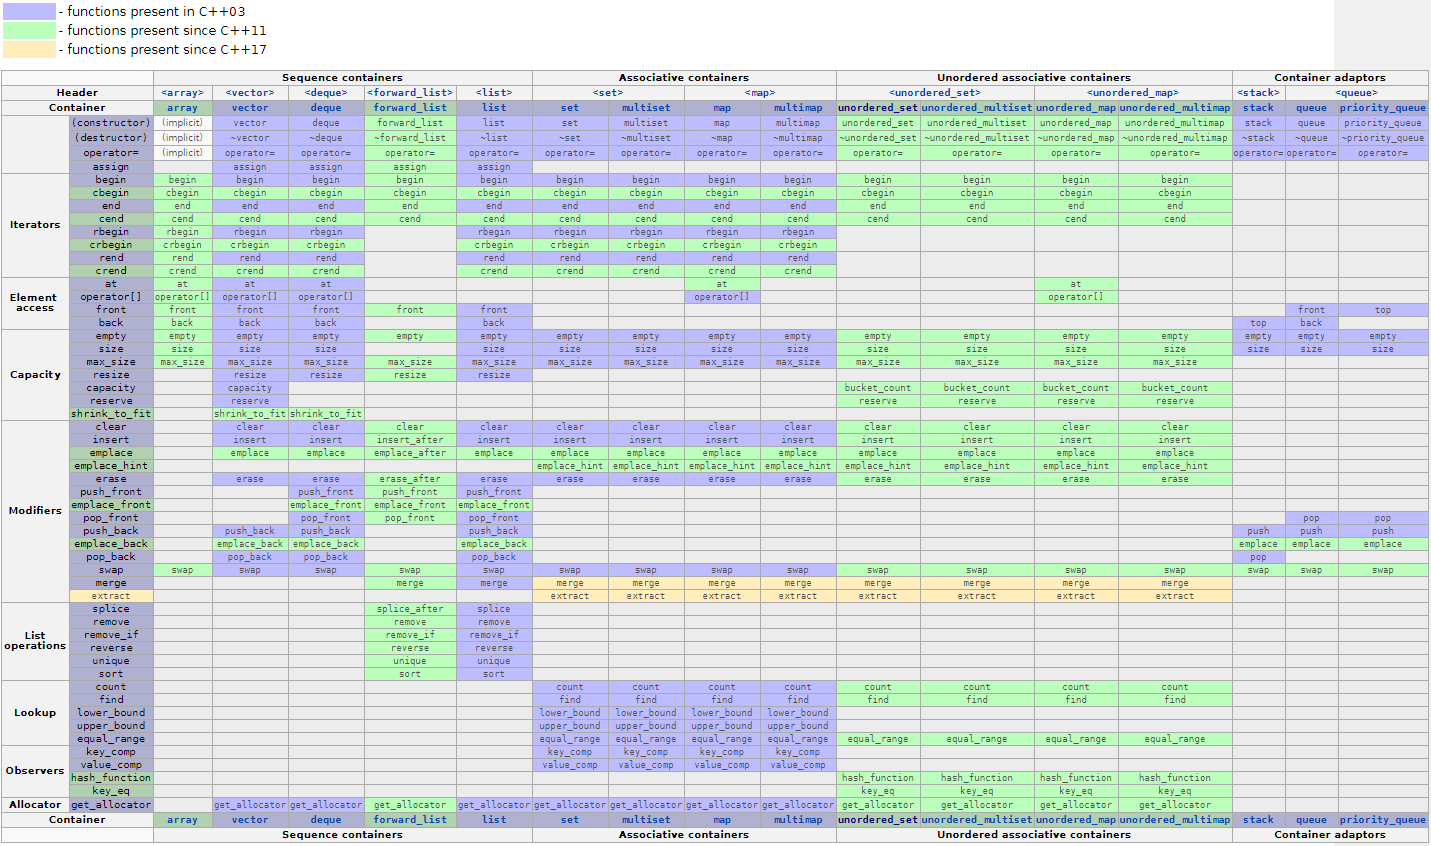
\includegraphics[width=\linewidth,clip,trim=0 6.3cm 15.5cm 0]{img/kontejnery-prehled-metod.png}
\end{frame}

\begin{frame}
% leva spodek prava vrsek
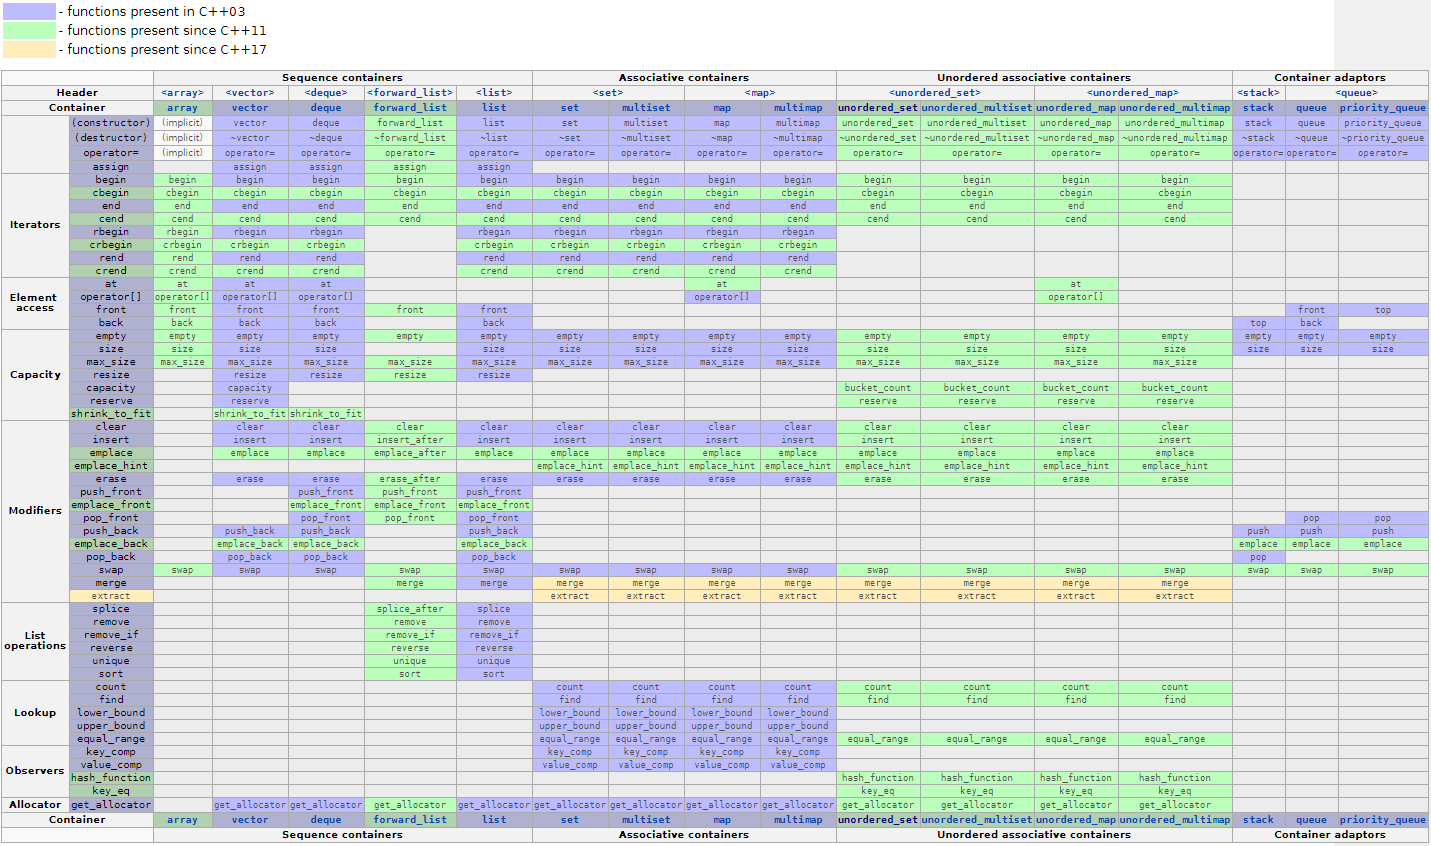
\includegraphics[width=\linewidth,clip,trim=0 0 15.5cm 15.9cm]{img/kontejnery-prehled-metod.png}
\end{frame}











\kapitola{Posloupnosti}

\begin{frame}[fragile]
\begin{block}{Přehled posloupností}
\begin{itemize}
\item \lstinline|array|\cpp{11} -- pole statické velikosti
\item \lstinline|vector| -- dynamicky alokované pole
\item \lstinline|deque| -- oboustranně dynamicky alokované pole
\item \lstinline|list| -- obousměrně zřetězený spojový seznam
\item \lstinline|forward_list|\cpp{11} -- jednosměrně zřetězený spojový seznam
\item adaptéry 
\begin{itemize}
\item \lstinline|stack| -- zásobník
\item \lstinline|queue| -- fronta
\item \lstinline|priority_queue| -- prioritní fronta
\end{itemize}
\end{itemize}
\end{block}
\end{frame}



\pkapitola{vector}

\begin{frame}[fragile]
\begin{block}{vector}
\begin{itemize}
\item \lstinline|#include <vector>|
\item šablona \lstinline|vector<TypDat, Alokator = vychozí>|
\item iterátor -- random access
\vskip 2ex
\item obvykle realizován jako dynamické pole
\vskip 2ex
\item poskytuje O(1) složitost čtení libovolného prvku
\item rychlé přidávání a odebírání prvků z konce vektoru
\item pomalá úprava prvků uprostřed vektoru
\end{itemize}
\end{block}
\end{frame}


\begin{frame}[fragile]
\begin{block}{vector}
\begin{itemize}
\item při úpravách pomalé realokace pole -- možnost rezervovat kapacitu vnitřního pole
\item \lstinline|vector.capacity()| -- vrací velikost interního pole
\item \lstinline|vector.reserve(velikost)| -- vyhradí paměť pro \lstinline|velikost| prvků
\item \lstinline|vector.resize(velikost)| -- změní počet prvků na \lstinline|velikost|, způsobuje smazání nebo přidání prvků!
\item \lstinline|vector.shrink_to_fit()|\cpp{11} -- zmenší vnitřní pole pouze na potřebnou velikost pro aktuální počet prvků
\end{itemize}
\end{block}
\end{frame}



\begin{frame}[fragile]
\frametitle{Vkládání hodnot}
\begin{yesblock}
\begin{lstlisting}
std::vector<int> v{};

// vložení hodnoty na konec
v.push_back(10);
// vložení hodnot na zvolené místo (iterátorem)
v.insert(v.end(), 20);

// konstrukce a vložení hodnoty na konci (C++11)
v.emplace_back(30);
// konstrukce a vložení hodnoty na zvoleném místě (C++11)
v.emplace(v.end(), 40);

for (auto item : v) { // foreach (C++11)
	cout << item << endl; 
}
// 10 20 30 40
\end{lstlisting}
\end{yesblock}
\end{frame}


\begin{frame}[fragile]
\frametitle{Vkládání hodnot -- objekt KomplexniCislo -- definice}
\begin{yesblock}
\begin{lstlisting}
struct KomplexniCislo {
	int real;
	int imag;

	KomplexniCislo() : real(0), imag(0) {}
	KomplexniCislo(int re, int im) : real(re), imag(im) {}
};

ostream& operator<<(ostream& os, const KomplexniCislo& kc) {
	os << kc.real << " + " << kc.imag << "i";
	return os;
}
\end{lstlisting}
\end{yesblock}
\end{frame}

\begin{frame}[fragile]
\frametitle{Vkládání hodnot -- objekt KomplexniCislo -- použití}
\begin{yesblock}
\begin{lstlisting}
std::vector<KomplexniCislo> v{};

v.push_back(KomplexniCislo{ 1, 0 });
v.insert(v.end(), KomplexniCislo{ 10, 0 });

v.emplace_back(1, 10);
v.emplace(v.end(), 5, 50);

vypis(v);
// 1 + 0i
// 10 + 0i
// 1 + 10i
// 5 + 50i
\end{lstlisting}
\end{yesblock}
\end{frame}


\begin{frame}[fragile]
\frametitle{Incializace pomocí initializer\_list}
\begin{yesblock}
\begin{lstlisting}
std::vector<KomplexniCislo> v{
	{1, 0},
	{10, 0},
	{1, 10},
	{5, 50}
};

vypis(v);
// 1 + 0i
// 10 + 0i
// 1 + 10i
// 5 + 50i
\end{lstlisting}
\end{yesblock}
\end{frame}

\begin{frame}[fragile]
\frametitle{Mazání prvků pomocí erase}
\begin{yesblock}
\begin{lstlisting}
std::vector<KomplexniCislo> v{
	{1, 0},
	{10, 0},
	{1, 10},
	{5, 50}
};

auto it = v.begin() + 1;
v.erase(it);

vypis(v);
// 1 + 0i
// - 10 + 0i - smazán
// 1 + 10i
// 5 + 50i
\end{lstlisting}
\end{yesblock}
\end{frame}

\begin{frame}[fragile]
\frametitle{Mazání prvků pomocí erase -- hromadné mazání}
\begin{yesblock}
\begin{lstlisting}
std::vector<KomplexniCislo> v{
	{1, 0},
	{10, 0},
	{1, 10},
	{5, 50}
};

auto it1 = v.begin() + 1;
auto it2 = v.begin() + 3;
v.erase(it1, it2);

vypis(v);
// 1 + 0i
// - 10 + 0i - smazán
// - 1 + 10i - smazán
// 5 + 50i
\end{lstlisting}
\end{yesblock}
\end{frame}




\begin{frame}[fragile]
\frametitle{Přístup k prvkům}
\begin{yesblock}
\begin{lstlisting}
std::vector<KomplexniCislo> v{
	{ 1, 0 },
	{ 10, 0 },
	{ 1, 10 },
	{ 5, 50 }
};

KomplexniCislo kc1 = v[0]; // 1 + 0i
KomplexniCislo kc2 = *v.begin(); // 1 + 0i
KomplexniCislo kc3 = *(v.begin() + 1); // 10 + 0i
KomplexniCislo kc4 = v.at(2); // 1 + 10i
KomplexniCislo kc5 = v.front(); // 1 + 0i
KomplexniCislo kc6 = v.back(); // 5 + 50i
KomplexniCislo kc7 = *v.rbegin(); // 5 + 50i
\end{lstlisting}
\end{yesblock}
\end{frame}






\pkapitola{deque}

\begin{frame}[fragile]
\begin{block}{deque}
\begin{itemize}
\item \lstinline|#include <deque>|
\item šablona \lstinline|deque<TypDat, Alokator = vychozí>|
\item iterátor -- random access
\vskip 2ex
\item obvykle realizován jako pole polí
\vskip 2ex
\item oproti vektoru zrychluje přidávání a odebírání prvků ze začátku kontejneru
\end{itemize}
\end{block}
\end{frame}


\begin{frame}[fragile]
\frametitle{Přidávání prvků na začátek/konec}
\begin{yesblock}
\begin{lstlisting}
std::deque<KomplexniCislo> d{
	{ 1, 0 },
	{ 10, 0 },
	{ 1, 10 },
	{ 5, 50 }
};

d.push_front({ 0, 0 });
// nebo také: d.emplace_front(0, 0);
d.push_back({ 100, 100 });
// 0 + 0i
// 1 + 0i
// 10 + 0i
// 1 + 10i 
// 5 + 50i
// 100 + 100i
\end{lstlisting}
\end{yesblock}
\end{frame}











\pkapitola{list}

\begin{frame}[fragile]
\begin{block}{list}
\begin{itemize}
\item \lstinline|#include <list>|
\item šablona \lstinline|list<TypDat, Alokator = vychozí>|
\item iterátor -- bidirectional
\vskip 2ex
\item obvykle realizován jako obousměrně zřetězený spojový seznam
\vskip 2ex
\item O(1) složitost libovolné atomické úpravy spojového seznamu
\item pomalé vyhledávání prvku
\item iterátor zůstává v platnosti i při změnách v seznamu
\end{itemize}
\end{block}
\end{frame}




\begin{frame}[fragile]
\begin{block}{Operace nad spojovým seznamem}
\begin{itemize}
\item \lstinline|l.remove(hodnota)| -- odebere všechny prvky s danou hodnotou
\item \lstinline|l.remove_if(podminka)| -- odebere všechny prvky splňující podmínku


\item \lstinline|l.unique()| -- odstraňuje po sobě jdoucí duplicitní prvky (\lstinline|==|)
\item \lstinline|l.unique(porovnavac)| -- dtto., umožňuje specifikovat metodu porovnávání prvků

\item \lstinline|l.splice(pozice, l2)| -- přesune všechny prvky z \lstinline|l2| před \lstinline|pozice|
\item \lstinline|l.splice(pozice, l2, pozicel2)| -- přesune vybraný prvek z \lstinline|l2| do \lstinline|l| na pozici \lstinline|pozice|
\item \lstinline|l.splice(pozice, l2, zacatekl2, konecl2)| -- přesune prvky z daného rozsahu před \lstinline|pozice|
\end{itemize}
\end{block}
\end{frame}




\begin{frame}[fragile]
\begin{block}{Operace nad spojovým seznamem\ldots}
\begin{itemize}
\item \lstinline|l.sort()| -- seřadí všechny prvky vzestupně (\lstinline|<|)
\item \lstinline|l.sort(porovnavac)| -- dtto., umožňuje specifikovat metodu porovnávání prvků


\item \lstinline|l.merge(l2)| -- sloučí dva seřazené seznamy
\item \lstinline|l.merge(l2, porovnavac)| -- dtto., umožňuje specifikovat metodu porovnávání prvků
\item \lstinline|l.reverse()| -- obrátí pořadí prvků
\end{itemize}
\end{block}
\end{frame}



\begin{frame}[fragile]
\frametitle{Odstranění prvků dle hodnoty}
\begin{yesblock}
\begin{lstlisting}
std::list<KomplexniCislo> l{
	{ 1, 0 },
	{ 10, 0 },
	{ 1, 10 },
	{ 10, 0 },
	{ 5, 50 }
};

l.remove({ 10, 0 });
// 1 + 0i
// 1 + 10i 
// 5 + 50i
\end{lstlisting}
\end{yesblock}
\end{frame}



\begin{frame}[fragile]
\frametitle{sort() a unique()}
\begin{yesblock}
\begin{lstlisting}
std::list<KomplexniCislo> l{
	{ 10, 0 }, { 1, 10 }, { 1, 0 }, { 10, 0 }, { 5, 50 }
};

l.sort(
	[](KomplexniCislo k1, KomplexniCislo k2) {
		if (k1.real == k2.real)
			return k1.imag < k2.imag;
		return k1.real < k2.real;
	}
);
l.unique();
// 1 + 0i
// 1 + 10i 
// 5 + 50i
// 10 + 0i
\end{lstlisting}
\end{yesblock}
\end{frame}



\begin{frame}[fragile]
\frametitle{Přesun prvků pomocí splice()}
\begin{yesblock}
\begin{lstlisting}
std::list<KomplexniCislo> dest{
	{ 0, 0 }, { 1, 0 }, { 1, 1 }, { 0, 1 }
};
std::list<KomplexniCislo> src{
	{ 5, 0 }, { 5, 0 }, { 5, 5 }, { 0, 5 }
};

auto destinationIterator = dest.begin(); // *it = {0, 0}
advance(destinationIterator, 1); // posun o 1 - *it = {1, 0}

auto sourceIterator = src.begin(); // *it = {5, 0}
advance(sourceIterator, 2); // posun o 2 - *it = {5, 5}

dest.splice(destinationIterator, src, sourceIterator);
// dest = { 0, 0 }, { 5, 5 }, { 1, 0 }, { 1, 1 }, { 0, 1 }
// src = { 5, 0 }, { 5, 0 }, { 0, 5 }
\end{lstlisting}
\end{yesblock}
\end{frame}











\kapitola{Asociativní kontejnery}



\begin{frame}[fragile]
\begin{block}{Přehled asociativních kontejnerů}
\begin{itemize}
\item struktury realizované nad vyvažovanými stromy
\begin{itemize}
\item \lstinline|set| -- množina prvků
\item \lstinline|multiset| -- dtto., může obsahovat duplicitní klíče
\item \lstinline|map| -- mapa (slovník - obsahuje dvojice klíč-hodnota)
\item \lstinline|multimap| -- dtto., může obsahovat duplicitní klíče
\end{itemize}
\item struktury realizované pomocí hashování
\begin{itemize}
\item \lstinline|unordered_set|\cpp{11} -- množina prvků
\item \lstinline|unordered_multiset|\cpp{11} -- dtto., může obsahovat duplicitní klíče
\item \lstinline|unordered_map|\cpp{11} -- mapa
\item \lstinline|unordered_multimap|\cpp{11} -- dtto., může obsahovat duplicitní klíče
\end{itemize}
\end{itemize}
\end{block}
\end{frame}





\begin{frame}[fragile]
\begin{block}{Základní vlastnosti asociativních kontejnerů}
\begin{itemize}
\item data jsou identifikována klíčem
\begin{itemize}
\item musí být definována operace pro porovnávání prvků
\item stromové struktury využívají standardně operaci \lstinline|operator<|
\item hashovací struktury využívají standardně operaci \lstinline|operator==|
\begin{itemize}
\item také musí být definována hashovací funkce převádějící klíč na celé číslo
\item knihovna obsahuje definici pro primitivní typy, string a některé další typy
\end{itemize}

\end{itemize}
\item klíč nelze změnit po vložení do struktury
\begin{itemize}
\item změnu je možné provést odebráním a přidáním prvku
\end{itemize}
\end{itemize}
\end{block}
\end{frame}


\pkapitola{set}

\begin{frame}[fragile]
\begin{block}{set}
\begin{itemize}
\item \lstinline|#include <set>|
\item šablona \lstinline|set<TypDat, KomparatorKlice = menšítko, Alokator = vychozí>|
\item iterátor -- bidirectional
\vskip 2ex
\item obvykle realizován vyvažovaný binární strom (AVL, Red-Black tree, \ldots)
\vskip 2ex
\item neposkytuje přímý přístup k prvkům
\item prvky jsou automaticky řazeny
\end{itemize}
\end{block}
\end{frame}


\begin{frame}[fragile]
\begin{block}{Operace nad množinou}
\begin{itemize}
\item \lstinline|s.count(klic)| -- vrací počet prvků s daným klíčem
\item \lstinline|s.find(klic)| -- vrací iterátor na první prvek s daným klíčem (nebo \lstinline|s.end()|)

\item \lstinline|s.lower_bound(klic)| -- vrací iterátor na první pozici, na kterou byl klíč vložen
\item \lstinline|s.upper_bound(klic)| -- vrací iterátor za poslední pozici, na kterou byl klíč vložen
\item \lstinline|s.equal_range(klic)| -- kombinuje předchozí dvě metody, vrací oba iterátory zároveň
\end{itemize}
\end{block}
\end{frame}

\begin{frame}[fragile]
\frametitle{Vyhledání prvku v množině}
\begin{yesblock}
\begin{lstlisting}
std::set<int> s{
	2, 5, 3, 1, 6, 9, 8, 7, 0
};

if (s.find(10) != s.end()) {
	cout << "Prvek 10 nalezen" << endl;
}
\end{lstlisting}
\end{yesblock}
\end{frame}












\begin{frame}[fragile]
\begin{block}{multiset}
\begin{itemize}
\item \lstinline|#include <set>|
\item šablona \lstinline|multiset<TypDat, KomparatorKlice = menšítko, Alokator = vychozí>|
\item iterátor -- bidirectional
\vskip 2ex
\item obvykle realizován vyvažovaný binární strom (AVL, Red-Black tree, \ldots)
\vskip 2ex
\item povoluje existenci duplicitních klíčů
\end{itemize}
\end{block}
\end{frame}


\begin{frame}[fragile]
\frametitle{Vyhledání prvků v multimnožině}

\begin{yesblock}
\begin{lstlisting}
std::multiset<int> s{
	2, 2, 1, 2, 3, 4, 5, 4, 4, 6, 7, 0, 9
};

auto iteratorPair = s.equal_range(4);
for (auto it = iteratorPair.first; it != iteratorPair.second; ++it) {
	cout << *it << endl;
}
// 4
// 4
// 4
\end{lstlisting}
\end{yesblock}
\end{frame}









\pkapitola{map}

\begin{frame}[fragile]
\begin{block}{map}
\begin{itemize}
\item \lstinline|#include <map>|
\item šablona \lstinline|map<TypKlice, TypDat, KomparatorKlice = menšítko, Alokator = vychozí>|
\item iterátor -- bidirectional
\vskip 2ex
\item obvykle realizován vyvažovaný binární strom (AVL, Red-Black tree, \ldots)
\vskip 2ex
\item tabulka obsahující dvojice klíč -- hodnota, klíče jsou po vložení do mapy neměnné, hodnoty lze měnit
\item přístup podle klíčů je rychlý
\item obsahuje obdobné operace jako množina pro přístup k datům
\end{itemize}
\end{block}
\end{frame}




\begin{frame}[fragile]
\frametitle{Vkládání hodnot do mapy}
\begin{yesblock}
\begin{lstlisting}
map<string, KomplexniCislo> m{};

m.insert(make_pair("pi", KomplexniCislo{ 3.1415, 0 }));
m.insert(make_pair("zero", KomplexniCislo{ 0, 0 }));

m.emplace("one", KomplexniCislo{ 1, 0 });
m.emplace("two", KomplexniCislo{ 2, 0 })
\end{lstlisting}
\end{yesblock}
\end{frame}



\begin{frame}[fragile]
\frametitle{Čtení hodnot z mapy}
\begin{yesblock}
\begin{lstlisting}
map<string, KomplexniCislo> m{
	{ "real", { 1, 0 } },
	{ "imag", { 0, 1 } }
};

// nalezení hodnoty - vrací iterátor (proto *)
std::pair<string, KomplexniCislo> p = *m.find("real");
// výpis komplexního čísla
cout << p.second;
\end{lstlisting}
\end{yesblock}
\end{frame}




\begin{frame}[fragile]
\begin{block}{}
\begin{itemize}
\item prvky je možné číst a zapisovat také pomocí přetíženého \lstinline|operator[]|
\begin{itemize}
\item čtení neexistujícího prvku tímto operátorem způsobí, že se prvek vytvoří v mapě!
\end{itemize}

\end{itemize}
\end{block}

\begin{yesblock}
\begin{lstlisting}
std::map<std::string, KomplexniCislo> komplexniKonstanty{};

komplexniKonstanty["imag"] = KomplexniCislo{0, 1};
komplexniKonstanty["real"] = KomplexniCislo{1, 0};
komplexniKonstanty["pi"] = KomplexniCislo{3.141592, 0};

std::cout << komplexniKonstanty["pi"];
\end{lstlisting}
\end{yesblock}
\end{frame}




\begin{frame}[fragile]
\begin{block}{multimap}
\begin{itemize}
\item \lstinline|#include <map>|
\item šablona \lstinline|multimap<TypKlice, TypDat, KomparatorKlice = menšítko, Alokator = vychozí>|
\item iterátor -- bidirectional
\vskip 2ex
\item obvykle realizován vyvažovaný binární strom (AVL, Red-Black tree, \ldots)
\vskip 2ex
\item oproti struktuře map umožňuje vkládat duplicitní klíče
\item neposkytuje přístup k prvků pomocí \lstinline|operator[]|
\end{itemize}
\end{block}
\end{frame}














\kapitola{Hashovací asociativní kontejnery\cpp{11}}


\begin{frame}[fragile]
\begin{block}{Přehled hashovacích asociativních kontejnerů}
\begin{itemize}
\item \lstinline|unordered_set|\cpp{11} -- množina prvků
\item \lstinline|unordered_multiset|\cpp{11} -- dtto., může obsahovat duplicitní klíče
\item \lstinline|unordered_map|\cpp{11} -- mapa
\item \lstinline|unordered_multimap|\cpp{11} -- dtto., může obsahovat duplicitní klíče
\end{itemize}
\end{block}
\end{frame}


\begin{frame}[fragile]
\begin{block}{Hashovací kontejnery}
\begin{itemize}
\item data nejsou v uspořádaném stromu, ale jsou organizována do \uv{buckets} dle hodnoty hashe
\item kontejnery poskytují operace pro prohlížení jednotlivých \uv{buckets} nebo pro rehashing kontejneru
\item iterátor -- forward
\item ostatní metody jsou shodné s nehashovacími variantami kontejnerů
\end{itemize}
\end{block}
\end{frame}


\begin{frame}[fragile]
\begin{block}{Parametry šablon hashovacích kontejnerů -- set}
\begin{itemize}
\item \lstinline|Key| -- typ dat množiny
\item \lstinline|Hash = std::hash<Key>| -- hashovací algoritmus
\item \lstinline|KeyEqual = std::equal_to<Key>| -- způsob porovnání klíčů
\item \lstinline|Allocator = std::allocator<Key>| -- typ alokátoru (pro nás nezajímavé)
\end{itemize}
\end{block}

\begin{block}{std::hash a std::equal\_to}
\begin{itemize}
\item realizovány jako šablony
\item definovány pro běžné primitivní typy, string, automatické ukazatele a další knihovní typy
\end{itemize}
\end{block}
\end{frame}


\begin{frame}[fragile]
\frametitle{Použití hashovacích kontejnerů}
\begin{yesblock}
\begin{lstlisting}
std::unordered_set<int> us{
	1, 2, 3, 4, 5, 6, 7, 8, 9, 10
};

for (auto i : us) {
	cout << i << endl;
}

// 9, 1, 2, 3, 4, 5, 6, 7, 8, 10
\end{lstlisting}
\end{yesblock}
\end{frame}


\begin{frame}[fragile]
\begin{yesblock}
\begin{lstlisting}[basicstyle=\small]
struct IntyHash {
	unsigned operator()(int value) const {
		return value % 3;
	}
};
struct IntyEqualTo {
	bool operator()(int v1, int v2) const {
		return v1 == v2;
	}
};
/////////////////////////////////////////////////////

std::unordered_set<int, IntyHash, IntyEqualTo> usv{
	1, 2, 3, 4, 5, 6, 7, 8, 9, 10
};

for (auto i : usv) {
	cout << i << endl;
}
// 10, 1, 4, 7, 2, 5, 8, 3, 6, 9
\end{lstlisting}
\end{yesblock}
\end{frame}
